\documentclass[12pt]{article}
 
\usepackage[margin=1in]{geometry} 
\usepackage{amsmath,amsthm,amssymb,outlines}
\usepackage{graphicx}
\usepackage{tikzsymbols}
\newenvironment{statement}[2][Statement]{\begin{trivlist}
\item[\hskip \labelsep {\bfseries #1}\hskip \labelsep {\bfseries #2.}]}{\end{trivlist}}
\newcommand{\littletaller}{\vphantom{\big|}}
\newcommand\restr[2]{{% we make the whole thing an ordinary symbol
  \left.\kern-\nulldelimiterspace % automatically resize the bar with \right
  #1 % the function
  \littletaller % pretend it's a little taller at normal size
  \right|_{#2} % this is the delimiter
  }}

\begin{document}
 
\title{Algebraic Topology Problem Bank} 
\author{Dahlen Elstran} 
\maketitle

\section{Revised}

\subsection{Homework 1}

\begin{statement}[Exercise]{0.2}
    Construct an explicit deformation retraction of $\mathbb{R}^n - \{0\}$ onto $S^{n-1}$.
\end{statement}
\begin{proof}
    First note that $S^{n-1}$ is defined to be all the points $(x_1, \dots, x_n)$ such that \\
    $\sqrt{x_1^2+ \dots + x_n^2}=1$. 
    Let $f_t(x_1, \dots , x_n)=(1+t(\frac{1}{\sqrt{x_1^2 + \dots + x_n^2}} - 1))(x_1, \dots, x_n)$. 
    Note that this is a continuous function because $(x_1, \dots, x_n) \neq 0$ and it is made up of 
    continuous functions. Then we have
    \begin{align*}
        f_0(x_1, \dots, x_n) &= (1+0)(x_1, \dots, x_n) = (x_1, \dots, x_n) \\
        f_1(x_1, \dots, x_n) &= (1 + \frac{1}{\sqrt{x_1^2 + \dots + x_n^2}} -1)(x_1, \dots, x_n) \\
        &= (\frac{1}{\sqrt{x_1^2 + \dots + x_n^2}})(x_1, \dots, x_n) \\
        &= (\frac{x_1}{\sqrt{x_1^2 + \dots + x_n^2}}, \dots, \frac{x_n}{\sqrt{x_1^2 + \dots + x_n^2}}).
    \end{align*}
    Notice that because 
    \begin{align*}
        & \sqrt{(\frac{x_1}{\sqrt{x_1^2 + \dots + x_n^2}})^2+ \dots + (\frac{x_n}{\sqrt{x_1^2 + \dots + x_n^2}})^2} \\
        & = \sqrt{\frac{x_1^2}{x_1^2 + \dots + x_n^2} + \dots + \frac{x_n^2}{x_1^2 + \dots + x_n^2}} \\
        & = \sqrt{\frac{x_1^2 + \dots + x_n^2}{x_1^2 + \dots + x_n^2}} = 1,
    \end{align*}
    we can conclude that $f_0(\mathbb{R}^n - \{0\})=\mathbb{R}^n - \{0\}$ and $f_1(\mathbb{R}^n - \{0\})=S^{n-1}$.
    Finally, let $(x_1, \dots, x_n) \in S^{n-1}$, so that $\sqrt{x_1^2+ \dots + x_n^2}=1$. Then 
    \begin{equation*}
        f_t(x_1, \dots, x_n)=(1+\frac{1}{\sqrt{x_1^2 + \dots + x_n^2}} - 1)(x_1, \dots, x_n) = 1 \cdot (x_1, \dots, x_n) =  (x_1, \dots, x_n).
    \end{equation*}
    So $\restr{f_t(x_1, \dots, x_n)}{S^{n-1}} = (x_1, \dots, x_n)$. Thus $f_t(x)$ is a deformation retraction.
\end{proof}

\begin{statement}[Exercise]{0.3}
    Before starting Exercise 0.3, let me state the following implications.    
\end{statement}
\begin{proof}
    First, note that for any continuous map $h$, $f \cong g \implies h(f) \cong h(g)$:
    \par Assuming $f \cong g$, there exists some continuous $\theta_t$ such that $\theta_0=f$ and $\theta_1=g$. Let $\theta'_t=h(\theta_t)$, and note that this is continuous because it is composed of continuous functions. Then $\theta'_0=h(\theta_0)=h(f)$, and similarly, $\theta'_1=h(\theta_1)=h(g)$. Thus $h(f) \cong h(g)$.
    \par Next, I aim to show that $f \cong g \implies f(h) \cong g(h)$:
    \par Assuming $f \cong g$, there exists some continuous $\theta_t$ such that $\theta_0=f$ and $\theta_1=g$. Let $\theta'_t=\theta_t(h)$, and note that this is continuous because it is composed of continuous functions. Then $\theta'_0=\theta_0(h)=f(h)$, and similarly, $\theta'_1=\theta_1(h)=g(h)$. Thus $f(h) \cong g(h)$.
\end{proof}
\begin{statement}[Exercise]{0.3a}
        Show that the composition of homotopy equivalences $X \to Y$ and $Y \to Z$ is a homotopy equivalence $X \to Z$. Deduce that homotopy equivalence is an equivalence relation.
\end{statement}
\begin{proof}
    First, to show the composition holds, assume that there is a homotopy equivalence from $X \to Y$, so there exists a continuous map $f_1: X \to Y$ such that there exists a continuous map $g_1: Y \to X$, and $f_1 \circ g_1 \cong \text{id}_y$ and $g_1 \circ f_1 = \text{id}_x$. Similarly, if there is a homotopy equivalence from $Y \to Z$, there exists a continuous map $f_2: Y \to Z$ such that there exists a continuous map $g_2: Z \to Y$, and $f_2 \circ g_2 \cong \text{id}_z$ and $g_2 \circ f_2 = \text{id}_y$.
    \par Define the following:
    \begin{align*}
        & f = f_2 \circ f_1 (x) = f_2(f_1(x)) \\
        & g = g_1 \circ g_2 (z) = g_1(g_2(z))
    \end{align*}
    Then $f$ and $g$ are continuous maps because they are composed of continuous functions, and 
    \begin{align*}
        (f \circ g)(z) &= f(g(z)) \\
        &= f_2(f_1(g_1(g_2(z)))) \\ 
        &= f_2(g_2(z)) = z \\ 
        (g \circ f)(x) &= g(f(x)) \\ 
        &= g_1(g_2(f_2(f_1(x)))) \\ 
        &= g_1(f_1(x))=x
    \end{align*}
    Thus $f$ is a homotopy equivalence from $X \to Z$. 
    \par Next we show that homotopy equivalence is an equivalence relation. 
    \par $\mathbf{Reflexivity}$: Let $f, g: X \to X$ be the identity map. Then $f,g$ are continuous, $f \circ g \cong \text{id}_x$, $g \circ f \cong \text{id}_x$. Thus $f$ is a homotopy equivalence, and $X \cong X$.
    \par $\mathbf{Symmetry}$: Assume $X \cong Y$. Then $f: X \to Y$ is a homotopy equivalence, so there exists $g: Y \to X$ such that $g \circ f \cong \text{id}_x$ and $f \circ g \cong \text{id}_y$. Let $f_0=g$ and $g_0=f$, so that $f_0:Y \to X$ is a continuous map, as is $g_0: X \to Y$; also, $g_0 \circ f_0 \cong \text{id}_y$ and $f_0 \circ g_0 \cong \text{id}_x$. Thus $Y \cong X$.
    \par $\mathbf{Transitivity}$: Assume $X \cong Y$ and $Y \cong Z$. Because $X \cong Y$, we know there exists $f_1:X \to Y$, $g_1:Y \to X$, $f_1 \circ g_1 \cong \text{id}_y$, and $g_1 \circ f_1 \cong \text{id}_x$. Similarly, because $Y \cong Z$, we know there exists $f_2:Y \to Z$, $g_2:Z \to Y$, $f_2 \circ g_2 \cong \text{id}_z$, and $g_2 \circ f_2 \cong \text{id}_y$. Then define 
    \begin{align*}
        & f = f_2 \circ f_1 \\
        &  g = g_1 \circ g_2,
    \end{align*}
    and note that both are continuous because they are composed of continuous functions. 
    \par Then 
    \begin{align*}
        & (f \circ g)(z) = f(g(z))=f_2(f_1(g_1(g_2(z))))=f_2(g_2(z))=z \\
        & (g \circ f)(x) = g(f(x))=g_1(g_2(f_2(f_1(x))))=g_1(f_1(x))=x.
    \end{align*}
    So $X \cong Z$ with $f$, so that transitivity is true, and a homotopy equivalence is an equivalence relation.
\end{proof}

\begin{statement}[Exercise]{0.3b}
    Show that the relation of homotopy among maps $X \to Y$ is an equivalence relation. 
\end{statement}
\begin{proof}
    \par $\mathbf{Reflexivity}$: Consider any $f: X \to Y$, and then let $f_t=f$, so that $f_0=f$ and $f_1=f$. Thus $f \cong f$.
    \par $\mathbf{Symmetry}$: Assume $f \cong g$, so that there exists a homotopy $f_t(x)$ such that $f_0=f$ and $f_1=g$. Define $f'_t(x)=f_{1-t}(x)$, and note that it is continuous. Then $f_0'(x)=f_1(x)=g$ and $f_1'(x)=f_0(x)=f$. Thus, by $f'_t(x)$, $g \cong f$.
    \par $\mathbf{Transitivty}$: Assume $f \cong g$ and $g \cong h$, so that there exists $\psi_t(x)$ such that $\psi_0=f$, $\psi_1=g$, and $\theta_t(x)$ such that $\theta_0=g$ and $\theta_1=h$. Define $\phi_t(x)$ as $\psi_{2t}(x)$ for $0 \leq t \leq \frac{1}{2}$ and $\theta_{2t-1}(x)$ for $\frac{1}{2} < t \leq 1$. Thus $\phi_t$ is continuous, because $\psi$ and $\theta$ are, and $\lim_{t \to \frac{1}{2}^-} \phi_t(x)=\psi_1(x)=g(x)=\theta_0(x)=\lim_{t \to \frac{1}{2}^+} \phi_t(x)$. Futhermore, $\phi_0= \psi_0=f$ and $\phi_1= \theta_1 = h$. Thus, $f \cong h$.
    \par Thus the relation of homotopy among maps is an equivalence relation.
\end{proof}

\begin{statement}[Exercise]{0.3c}
    Show that a map homotopic to a homotopy equivalence is a homotopy equivalence. 
\end{statement}
\begin{proof}
    Let $f: X \to Y$ be a homotopy equivalence, and assume it is homotopic to $g: X \to Y$. Because $f$ is a homotopy equivalence, there exists some continuous $h: Y \to X$ such that $f \circ h \cong \text{id}_y$ and $h \circ f \cong \text{id}_x$. Because $h$ is continuous, we can use a previous result to say that because $f \cong g$, then $h(f) \cong h(g)$. Because $f(h) \cong \text{id}_y$, by transitivity proven above, $h(g) \cong \text{id}_y$. Similarly, we can also say that $f(h) \cong g(h)$, and so because $f(h) \cong \text{id}_y$, then $g(h) \cong \text{id}_y$. Thus $g$ is homotopy equivalent. 
\end{proof}

\begin{statement}[Exercise]{0.10}
    Show that a space $X$ is contractible if and only if every map $f:X \to Y$, for arbitrary $Y$, is nullhomotopic. Similarly, show $X$ is contractible if and only if every map $f: Y \to X$ is nullhomotopic.
\end{statement}
\begin{proof}
    Assume $X$ is contractible. Then we know any identity map $h: X \to X$ is nullhomotopic. Then we know, because $h \cong g$ for constant function $g$, that $f(h) \cong f(g)$, and $f(h)=h$ and $f(g)=g_0$, a constant function. Thus $f$ is nullhomotopic for any $Y$. 
    \par Assume every map $f:X \to Y$, for arbitrary $Y$, is nullhomotopic. Then the identity map $f: X \to X$ is nullhomotopic. Thus, by definition, $X$ is contractible.
    \par For the more general statement, first assume $X$ is contractible, so that $h:X \to X$, $h \cong g$ (where $g$ is a constant function). Let $f: Y \to X$ be a map with any space $Y$. Then there exists $f_t(x)$ such that $f_0=h$, and $f_1=g$. Let $f'_t=f_t(f)$ (and note that $f'_t(x)$ is still continuous), so $f_0'=h(f)$, and $f'_1 \cong g_1(f)$. Then $f \cong g_1(f)$, and $g_1(f)$ is a constant function.
    \par Assume every map $f: Y \to X$ is nullhomotopic, then $f: X \to X$, where $f$ is the identity function, is nullhomotopic, and therefore $X$ is contractible. 
\end{proof}

\begin{statement}[Exercise]{0.11}
    Show that $f: X \to Y$ is a homotopy equivalence if there exist maps $g,h:Y \to X$ such that $fg \cong \text{id}$ and $hf \cong \text{id}$. More generally, show that $f$ is a homotopy equivalence if $fg$ and $hf$ are homotopy equivalences. 
\end{statement}
\begin{proof}
    Assume there exists $g,h: Y \to X$ such that $fg \cong \text{id}_y$, $hf \cong \text{id}_x$. Then, because $fg \cong \text{id}_y$, we know $fgf \cong f \iff fgf \cong f \circ \text{id}_x$. Then $gf \cong \text{id}_x$, and so for $f:X \to Y$, there exists $g: Y \to X$ such that $fg \cong \text{id}_y$ and $hf \cong \text{id}_x$, so $f:X \to Y$ is a homotopy equivalence. 
    \par Assume that there exists $h,g: Y \to X$, and $fg$ and $hf$ are homotopy equivalents. Then we know
    \begin{align*}
        & fg \text{ is homotopy equivalent } \iff \exists g':Y \to Y, fg \circ g' \cong \text{id}_y, g' \circ fg \cong \text{id}_y \\
        & hf \text{ is homotopy equivalent } \iff \exists h':X \to X, hf \circ h' \cong \text{id}_x, h' \circ hf \cong \text{id}_x
    \end{align*}
    Then we have
    \begin{align*}
        h'hf \cong \text{id}_x & \implies h(fh'h) \cong \text{id}_x \circ h \cong h \cong h \circ \text{id}_x \\
        & \implies fh'h \cong \text{id}_x \cong h'hf
    \end{align*}
    So because of $h'h$, $f$ is a homotopy equivalence. 
\end{proof}

\begin{statement}[Exercise]{0.17a}
    Show that the mapping cylinder of every map $f:S^1 \to S^1$ is a CW complex. 
\end{statement}
\begin{proof}
    Let $f:S^1 \to S^1$ be any arbitrary mapping. To construct the CW complex, start with two 0-cells, $e^0_1$, acting as an $x$ coordinate, and $e_2^0$, acting as it's $y$ coordinate. Then add the 1-cell $e^1_1$ as a circle, where $e^0_1$ is in this circle, and another 1-cell $e^1_2$ as another (disjoint) circle, this time with $e^1_2$ containing $e^0_2$. Then add one more 1-cell, $e^1_3$, as the graph of $f$, effectively going around the cylinder. Finally, attach a 2-cell $e^2_1$ so that it "closes" the cylinder. An attempted diagram is attached below:
    \par 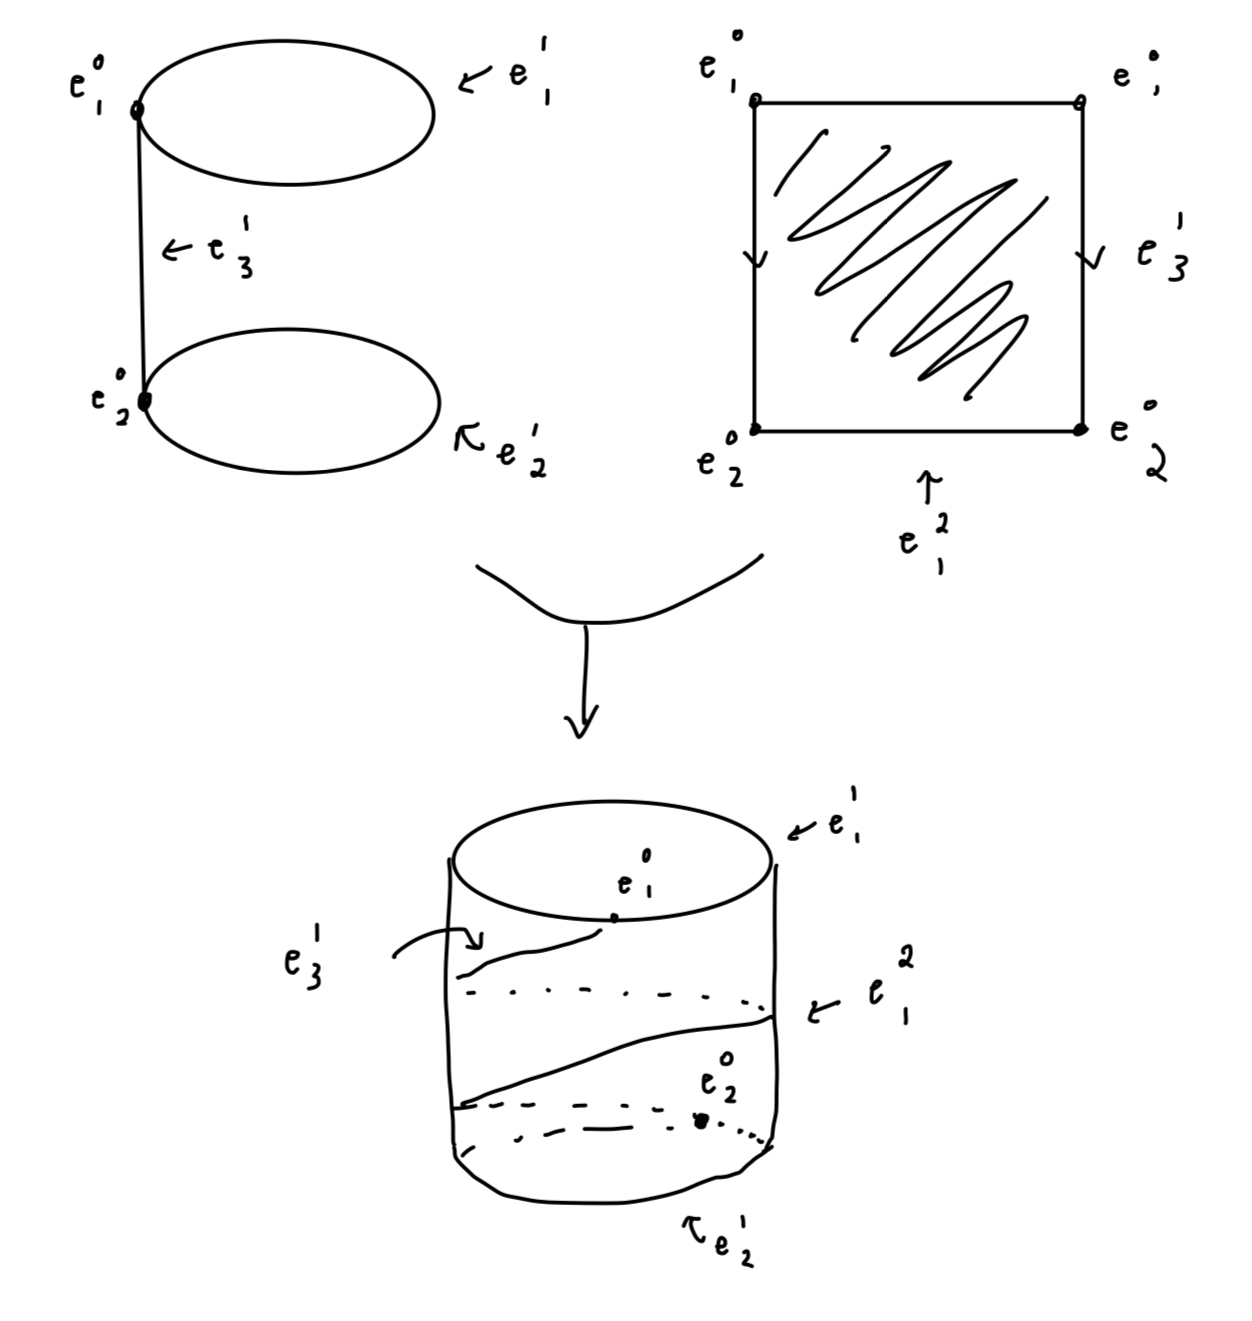
\includegraphics[scale=.3]{1.17.1.jpg}
\end{proof}

\begin{statement}[Exercise]{0.17b}
    Construct a 2-dimensional CW complex that contains both an annulus $S^1 \times I$ and a Mobius band as deformation retracts. 
\end{statement}
\begin{proof}
    Both the Mobius band and the annulus can deformation retract onto their middle circles, so if we glue the middle circles together, we can get a 2-dimensional CW complex that can deformation retract to both. Image below:
    \par 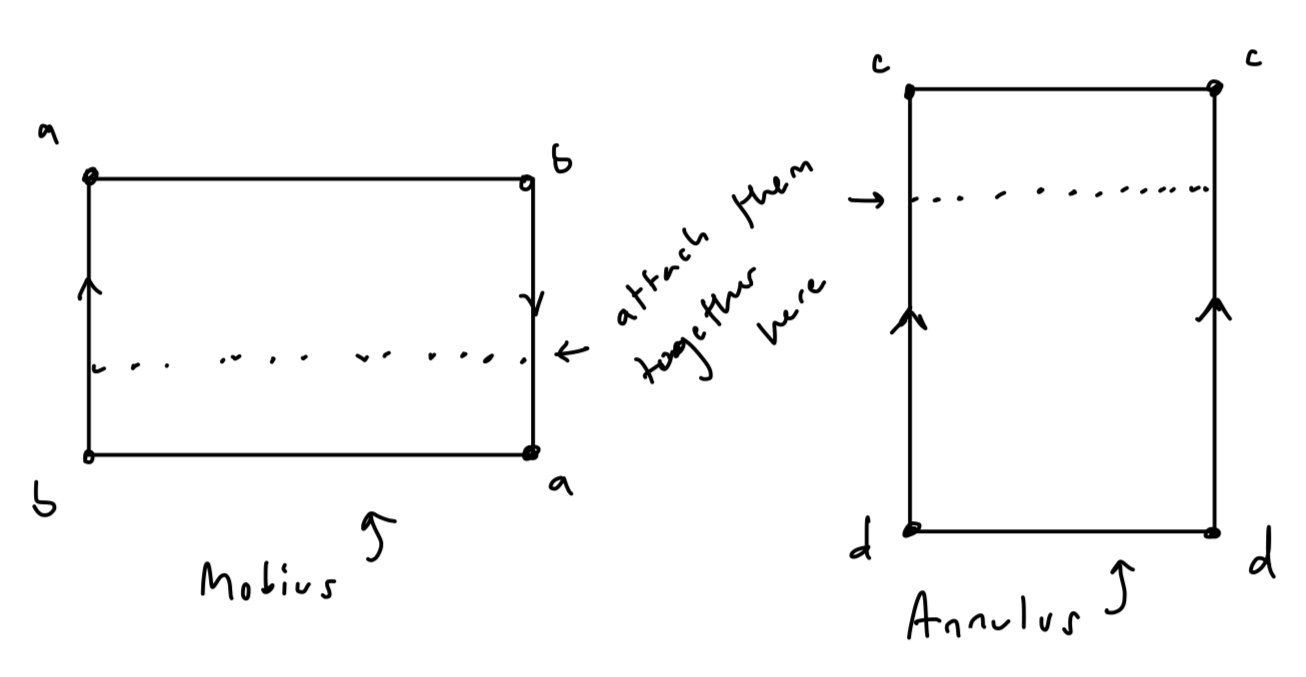
\includegraphics[scale=.3]{1.17.2.jpg}
\end{proof}

\begin{statement}[Exercise]{0.20}
    Show that the subspace $X \subset \mathbb{R}^3$ formed by a Klein bottle intersecting itself in a circle is homotopy equivalent to $S^1 \vee S^1 \vee S^1$.
\end{statement}
\begin{proof}
    As shown in the picture below, you can condense there the neck meets the rest of the bottle into one point, extend the neck out so there is only a 1-cell coming from that intersection point, until the neck is pushed all the way into a sphere. Then all that is left is a sphere with a circle on the outside and another cirlce on the inside, where the circles intersect at exactly one point. Thus $X \subset \mathbb{R}^3 \cong S^1 \vee S^1 \vee S^1$.
    \par 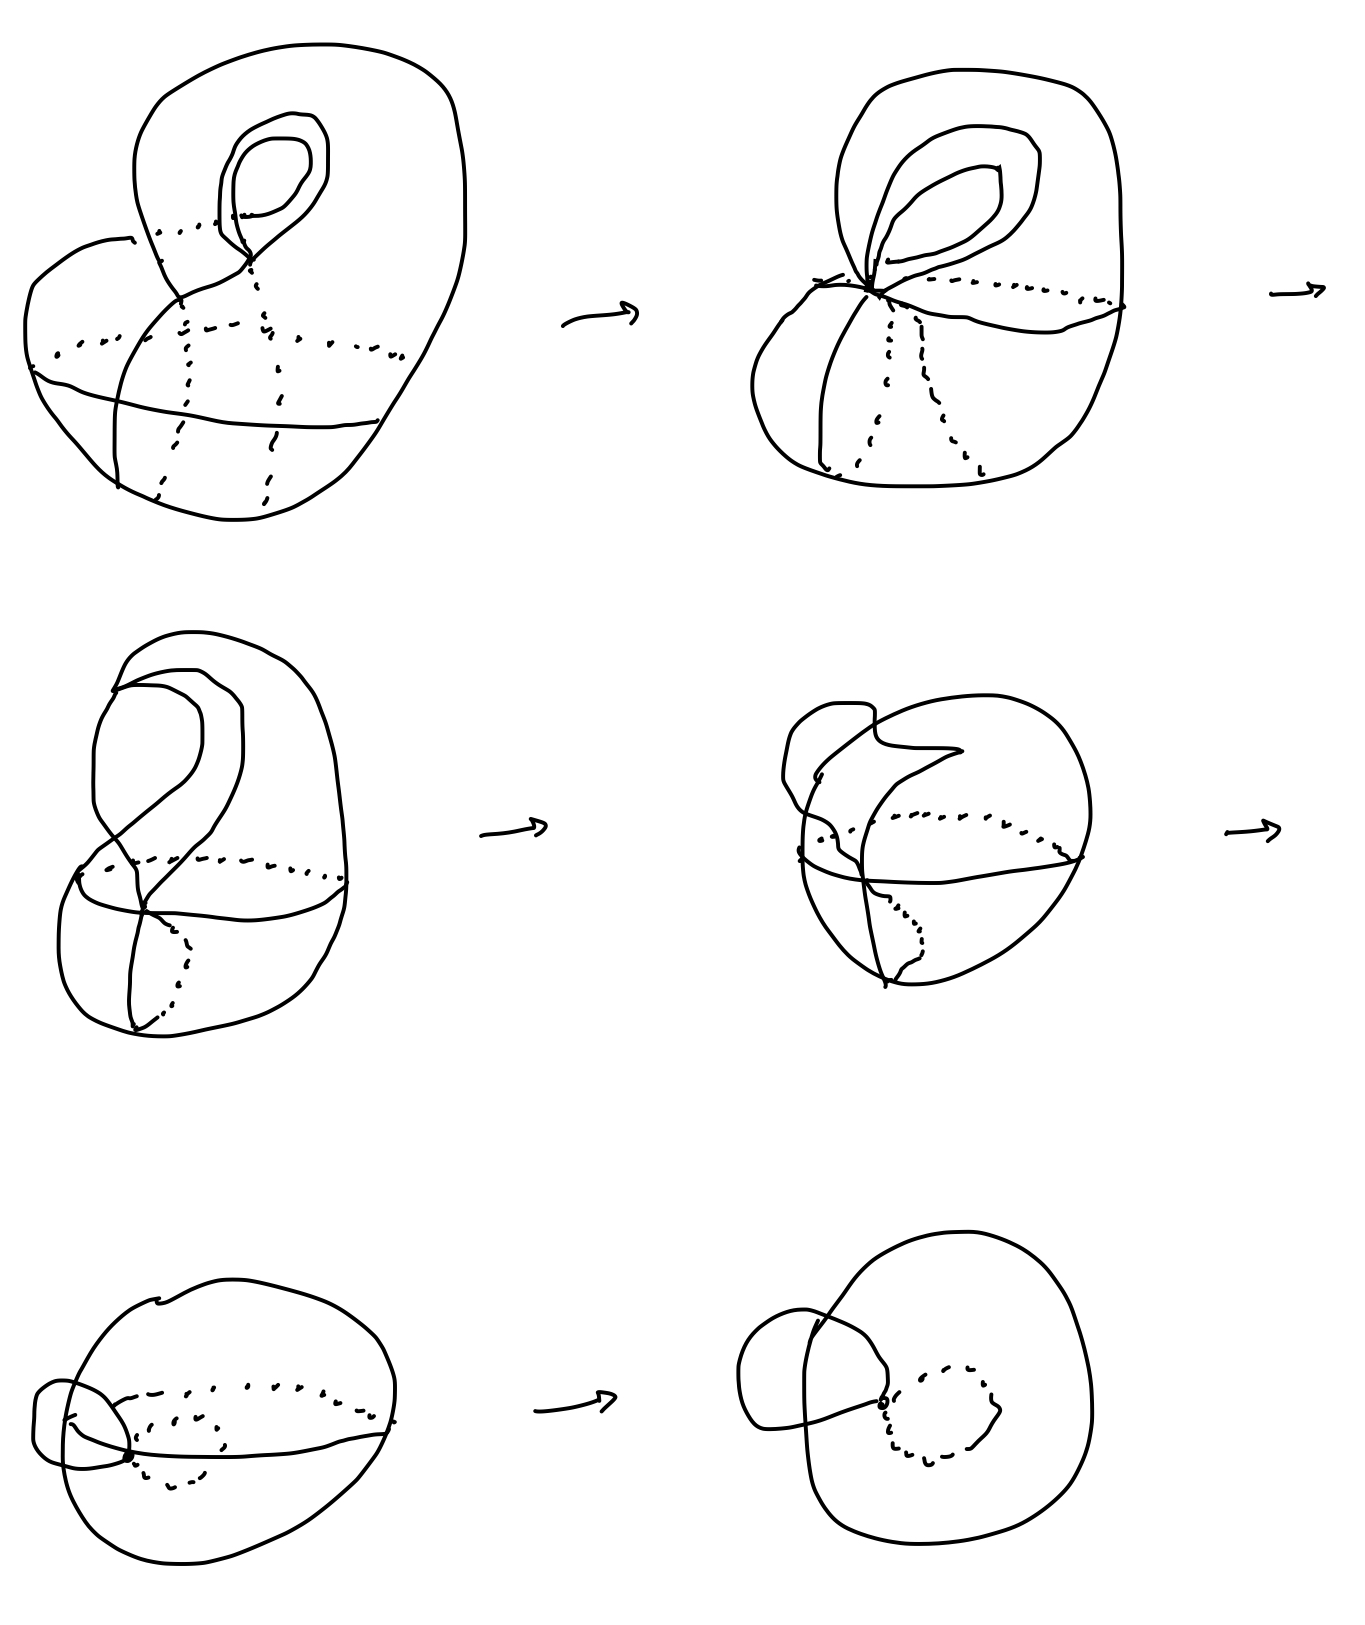
\includegraphics[scale=.3]{1.20.jpg}
\end{proof}

\subsection{Homework 1 Extra Problems}

\begin{statement}[Hatcher] {0.6}
  \begin{itemize}
    \item Let $X$ be the subspace of $\mathbb{R}^2$ consisting of the horizontal segment $[0,1] \times \{0\}$ together with all the vertical segments 
      $\{r\} \times [0,1-r]$. 
  \end{itemize}
\end{statement}

\section{Not Revised}

\subsection{Homework 2}

\begin{statement}[Exercise]{1}
    Describe a CW complex structure on $\mathbb{C}P^2 \times \mathbb{R}P^2$ and $\Sigma T^2$.
\end{statement}
\begin{proof}
    For $\mathbb{C}P^2 \times \mathbb{R}P^2$, we know that $\mathbb{R}P^2$ consists of 1 0-cell, 1 1-cell, and 1 2-cell. Similarly, for $\mathbb{C}P^2$, it consists of 1 1-cell, 1 2-cell, and 1 4-cell. Thus the product of these spaces consists of 1 0-cell, 1 1-cell, 2 2-cell, 1 3-cell, 2 4-cell, 1 5-cell, and 1 6-cell. Visually, we're finding the product of a sphere and a 4th dimensional shape.
    \par For $\Sigma T^2$, first note that $T^2 = S^1 \times S^1$, the torus. In Hatcher, it is stated that $\Sigma X = X \wedge S^1$, so in our case, $\Sigma (S^1 \times S^1) = (S^1 \times S^1) \wedge S^1$. Also in Hatcher, $ X \wedge Y = X \times Y / X \vee Y$. So finally, we have $ (S^1 \times S^1) \times S^1 / (S^1 \times S^1) \vee S^1$. Visually, we can imagine this as a torus crossed with $S^1$ quotient by a torus touching a circle. Regarding cell complexes, we have $(e^0 \cup e^1 \cup e^1 \cup e^1 \cup e^2 \cup e^2 \cup e^2 \cup e^3) / (e^0 \cup e^0 \cup e^1 \cup e^1 \cup e^1 \cup e^2)$. Thus the reduced suspension of a torus has the CW structure of 1 1-cell, 2 2-cells, and 1 3-cell.
\end{proof}

\begin{statement}[Exercise]{2}
    Let $X_n$ be the topological space obtained by identifying $n > 1$ points on $S^2$ to a single point. Describe a CW decomposition of $X_n$.
\end{statement}
\begin{proof}
    When you identify a point with a singular point, you're pinching the $S^2$ sphere at that singular point, and it creates a "loop" from where the point originally was to the singular point. This occurs for every point identified, so that there are $n-1$ loops (or $S^1$'s) added to the space. Note that we need loops, because if we were to do lines, some lines could intersect. Thus we can say $X_n = S^2 \vee \bigvee_{i=1}^{n-1} S^1$, which is just stating that $X_n$ is a sphere with loops added that intersect at a single point (the singular point). When considering CW decomposition, the $S^2$ has 1 0-cell and 1 2-cell, while each $S^1$ has a 0-cell and a 1-cell. However, the singular point can be made the 0-cell for the $S^2$ and the $S^1$'s, so in total there is 1 0-cell, 1 2-cell, and $n-1$ 1-cells. 
\end{proof}

\begin{statement}[Exercise]{3}
    Hatcher Exercise 0.21: If $X$ is a connected Hausdorff space that is a union of a finite number of 2-spheres, any two of which intersect in at most one point, show that $X$ is homotopy equivalent to a wedge sum of $S^1$'s and $S^2$'s.
\end{statement}
\begin{proof}
    First, because the space is connected, we know that there aren't any disjoint 2-spheres. Then, we can imagine this space made up of $S^2$'s which intersect at most 1 point, and because there can't be any disjoint 2-spheres, they must all be in a row like this, or in a loop:
    \par 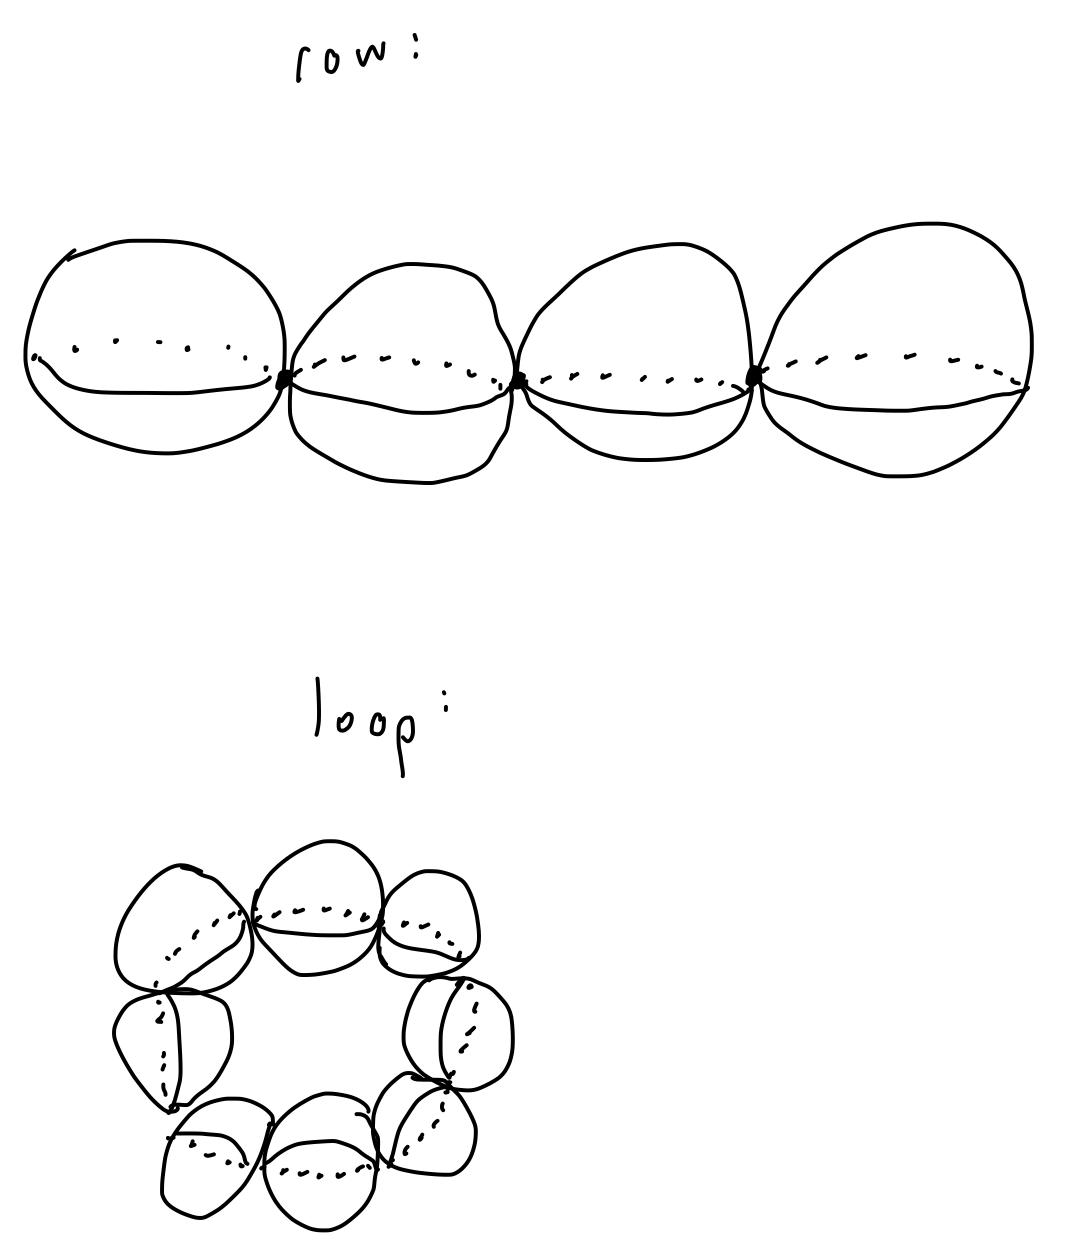
\includegraphics[scale=.2]{2.3.1.png}
    \par Either way, the intersection points between the spheres can be stretched into lines between them, like this:
    \par 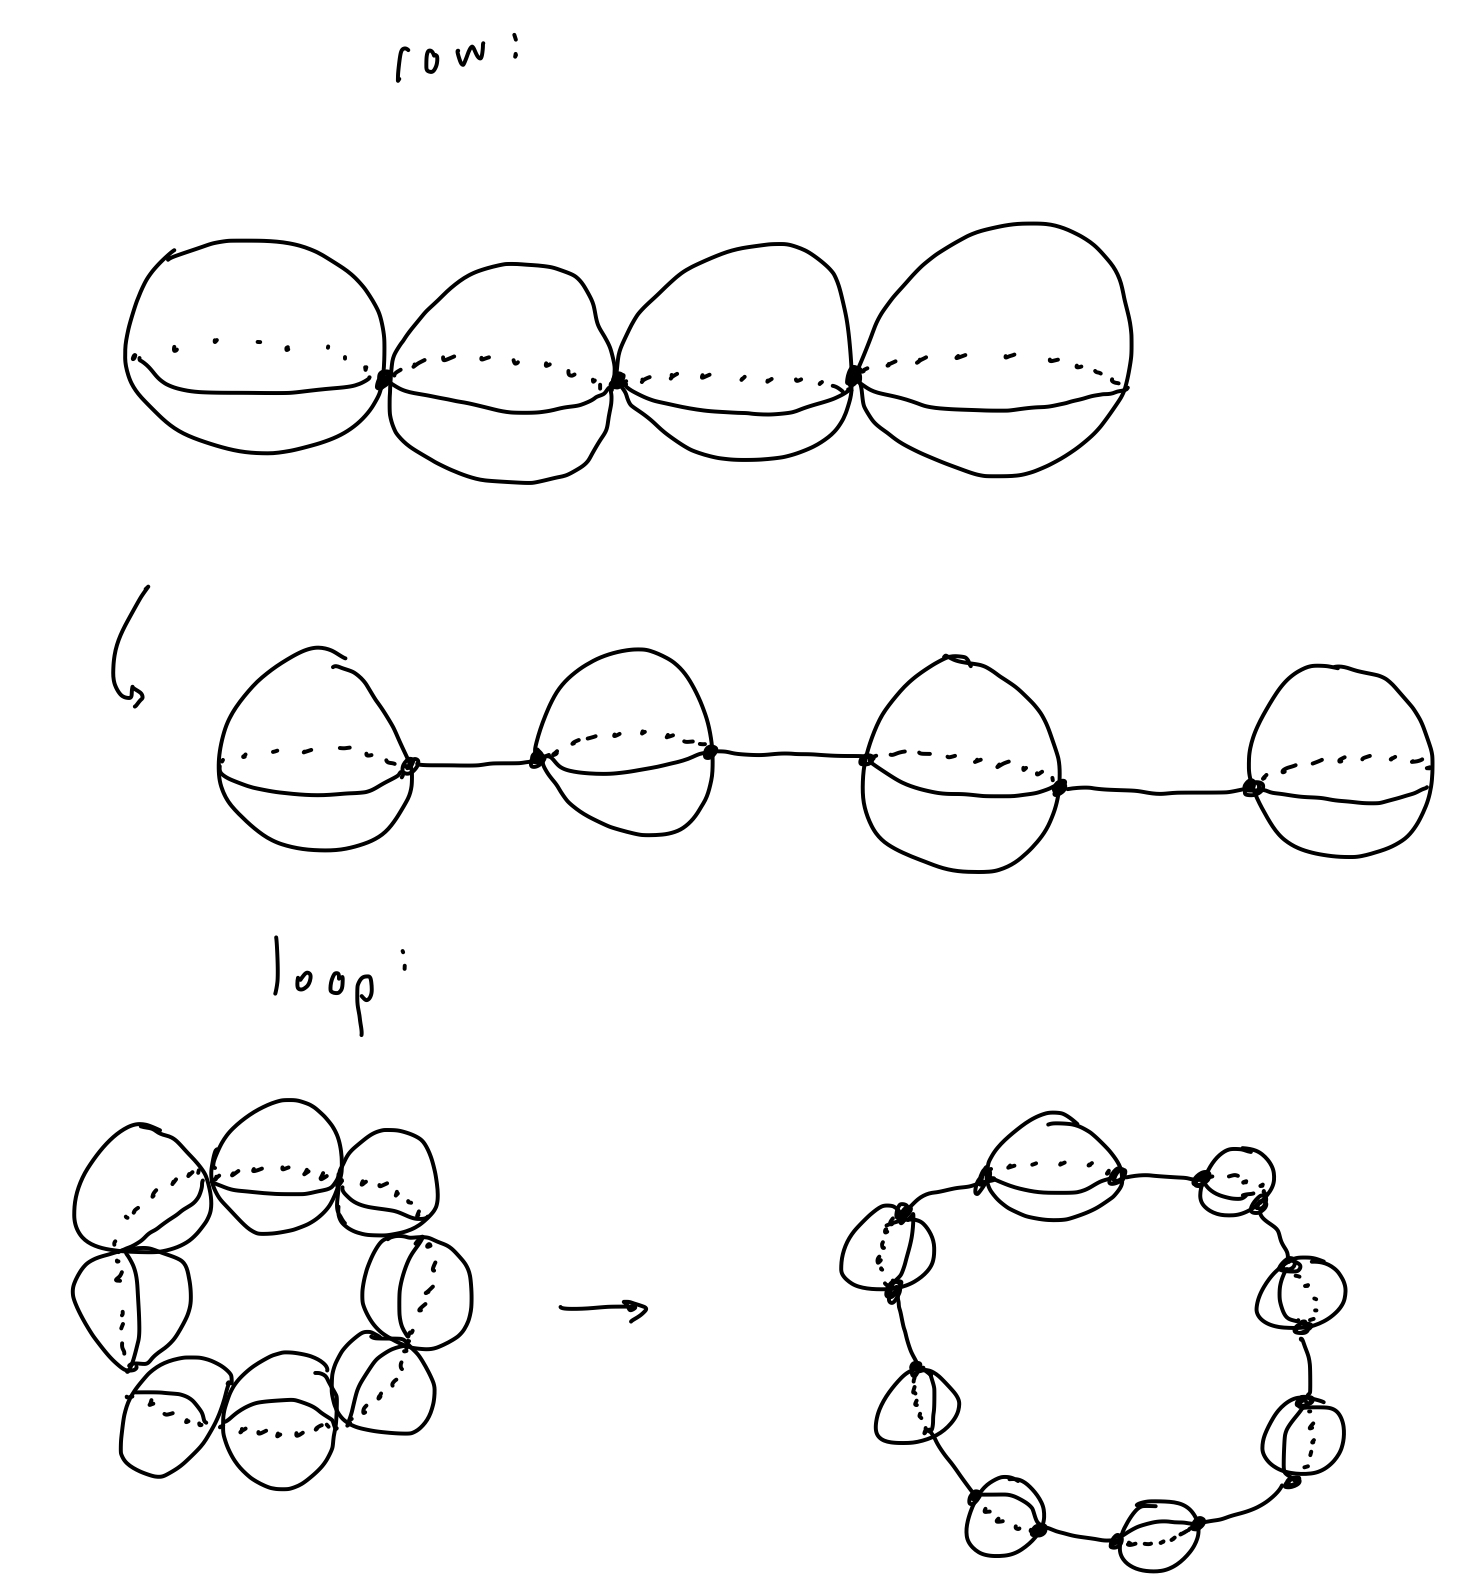
\includegraphics[scale=.2]{2.3.2.png}
    \par As you can see, the space $X$ can be stretched (and is therefore homotopically equivalent to) to be $\bigvee_{i=1}^{n-1} S^1 \vee \bigvee_{i=1}^{n} S^2$ where $n$ is the number of 2-sphere's in $X$. 
\end{proof}

\begin{statement}[Exercise]{4}
    Hatcher Exercise 0.25: If $X$ is a CW complex with components $X_{\alpha}$, show that the suspension $SX$ is homotopy equivalent to $Y \vee_{\alpha} SX_{\alpha}$ for some graph $Y$. In the case that $X$ is a finite graph, show that $SX$ is homotopy equivalent to a wedge sum of circles and 2-spheres. 
\end{statement}
\begin{proof}
    If $X$ is a finite graph, the suspension $SX$ is just taking all the vertices in the graph and connecting them to a point "above" and "below" the graph. This results in something like this: 
    \par 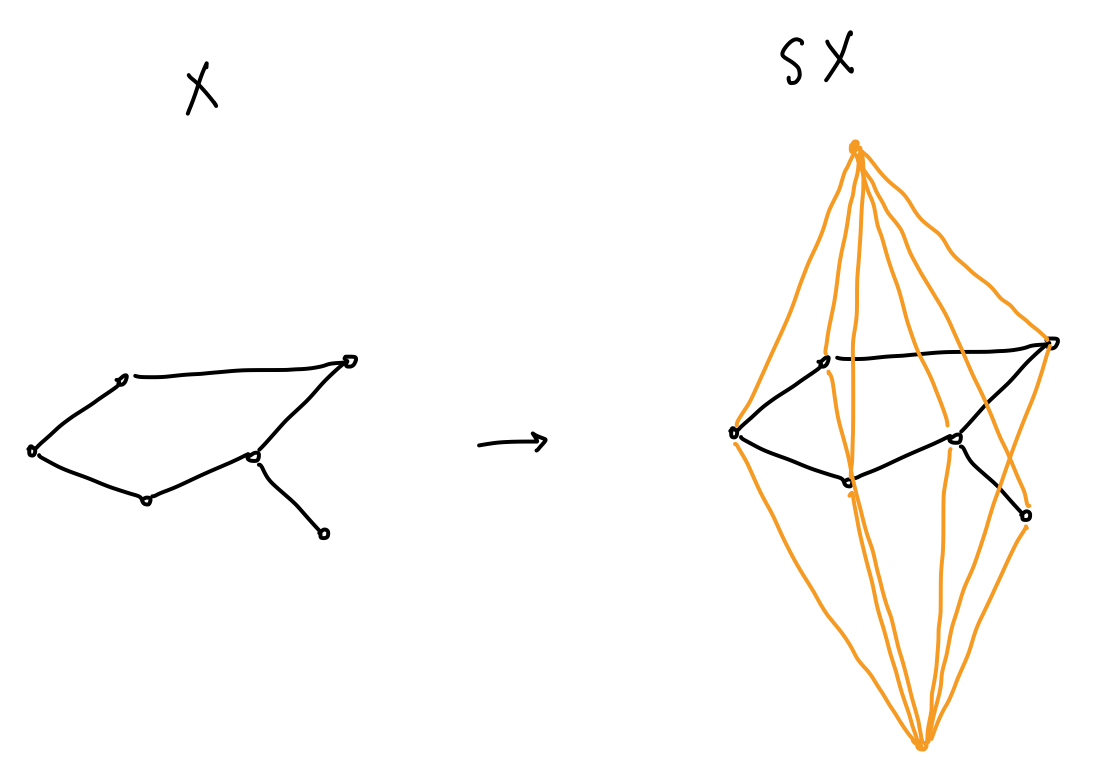
\includegraphics[scale=.2]{2.4.1.png}
    \par Note that when you have a closed loop in a graph, when you do the suspension it results in a sphere, and when there is a non-loop, it just creates circles:
    \par 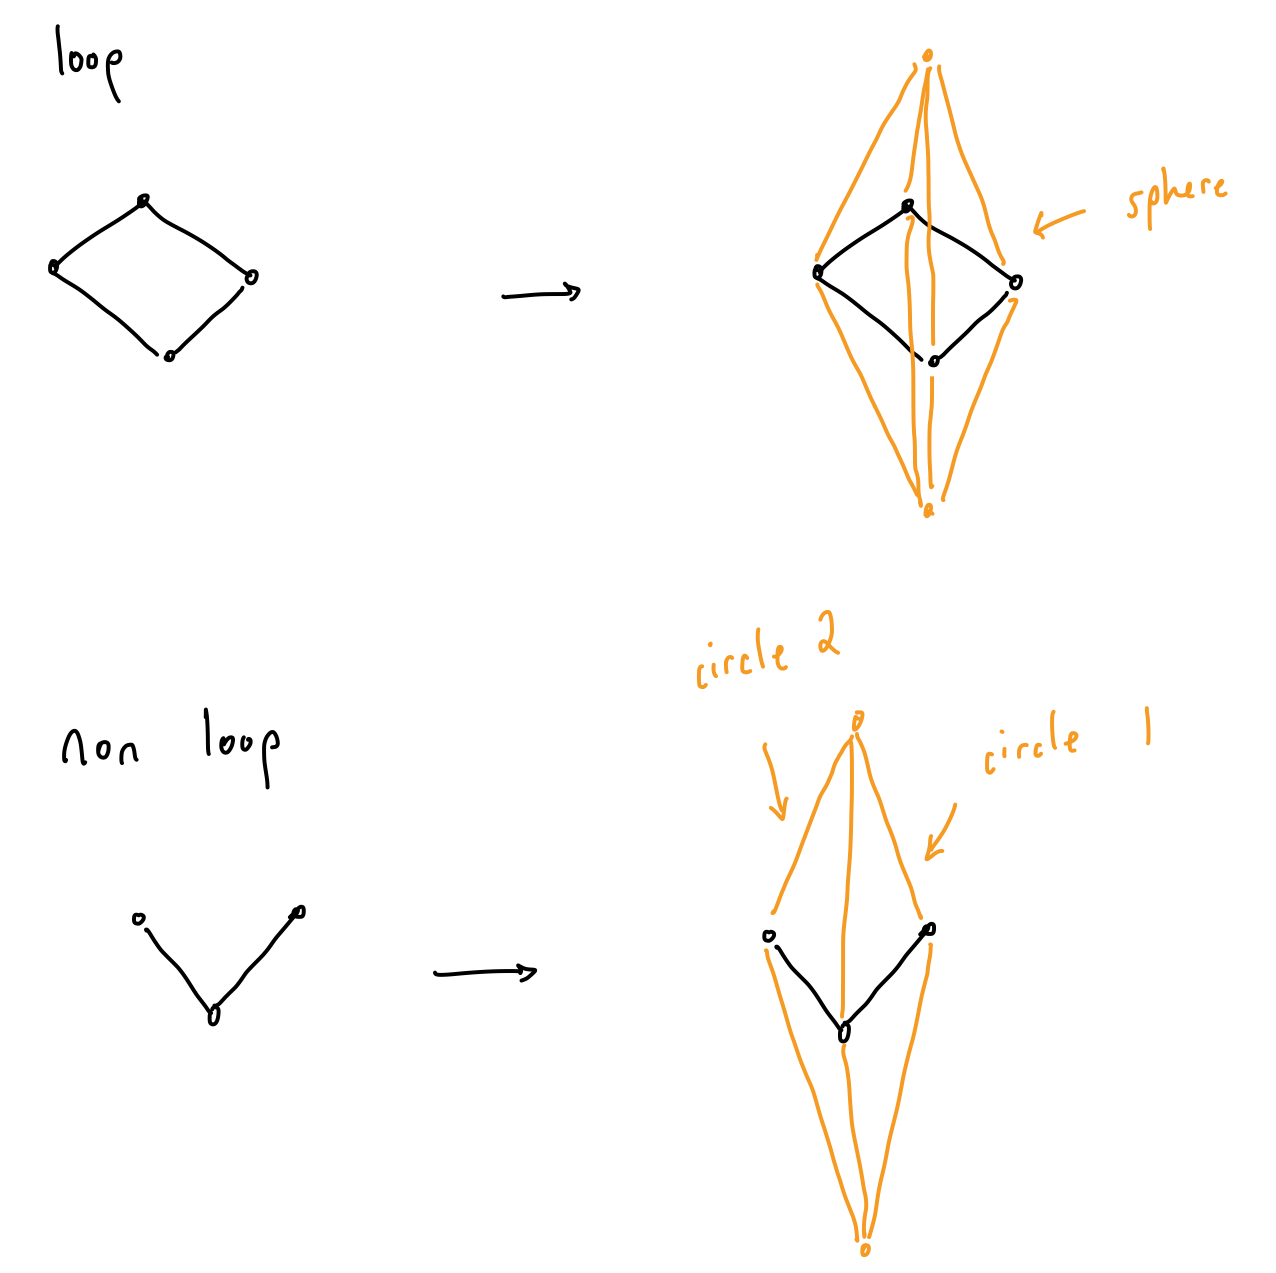
\includegraphics[scale=.2]{2.4.2.png}
    \par Because everything in a graph is either a loop or a nonloop, this accounts for what makes up any graph $X$. Thus if $X$ is a graph, $SX$ is just a wedge sum of spheres and circles. 
\end{proof}

\end{document}
